% !TeX spellcheck = de_DE
\section{Evaluation}
\label{sec:evaluation_parallel}
Nachdem die Parallelisierung der Evaluationsphase durchgeführt und die Testumgebung spezifiziert ist, wird in diesem Kapitel die Performance des Verfahrens gemessen. Die hierbei erhaltenen Ergebnisse werden mit denen der sequenziellen Implementierung verglichen. Im letzten Schritt wird eine Bewertung bezüglich der Effizienz und des \emph{SpeedUps} abgegeben.

\subsection{MountainCar}
\label{subsec:mountain_car_optimzation}
Das parallelisierte Verfahren wird zuerst in der \emph{MountainCar} Umgebung getestet, die aus Kapitel \ref{subsec:analysis_mountain_car} bekannt ist. Mit dem Ziel, einen einfachen Vergleich zwischen der sequenziellen und parallelisierten Implementierung zu ermöglichen, wird die zuvor verwendete Konfiguration des Verfahrens vollständig übernommen. Selbiges gilt für den \emph{Seed}. Bei korrekter Implementierung des parallelisierten Verfahrens werden dieselben Zwischenergebnisse nach jeder Generation generiert und das finale Ergebnis stimmt mit dem des sequenziellen Verfahrens überein. Somit kann keine Implementierung einen zeitlichen Vorteil erlagen, der durch bessere Agenten oder kürzere Evaluationszeiten entsteht. Beide Implementierungen werden dieselben Berechnungen und Evaluationen durchführen.
\begin{figure}[!h]
	\centering
	\begin{minipage}[]{0.49\textwidth}
		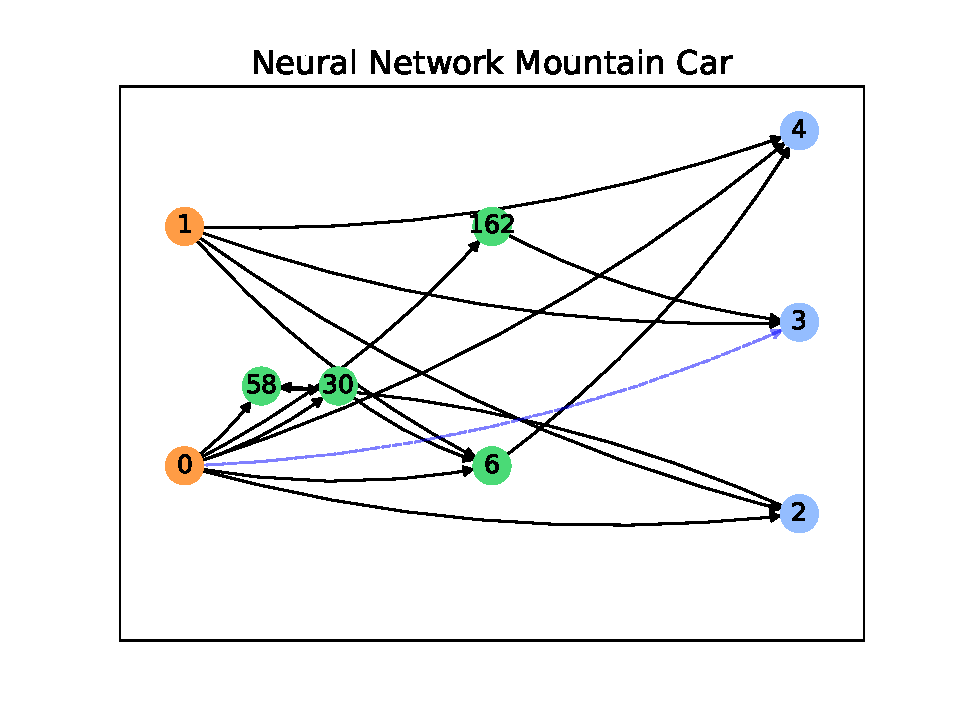
\includegraphics[width=1.0\textwidth]{./img/mountain_car_single/mountain_car_neural_network.pdf} 
	\end{minipage}
	\hfill
	\begin{minipage}[]{0.49\textwidth}
		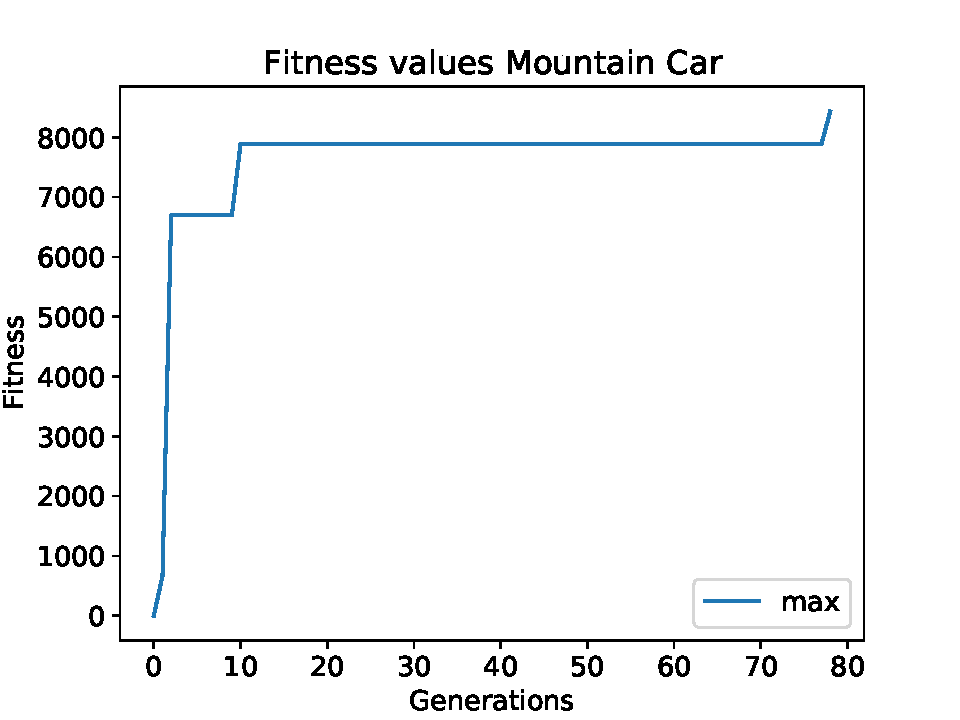
\includegraphics[width=1.0\textwidth]{./img/mountain_car_single/1413_fitness_1core_1pi.pdf} 
	\end{minipage}
	\caption{Links die Lösung für das \emph{MountainCar} Problem, rechts die dazugehörigen Fitnesswerte pro Generation mit 10 Prozessen}
	\label{fig:mountain_car_10core_neural_network_and_fitness}
\end{figure}
\begin{figure}[!h]
	\centering
	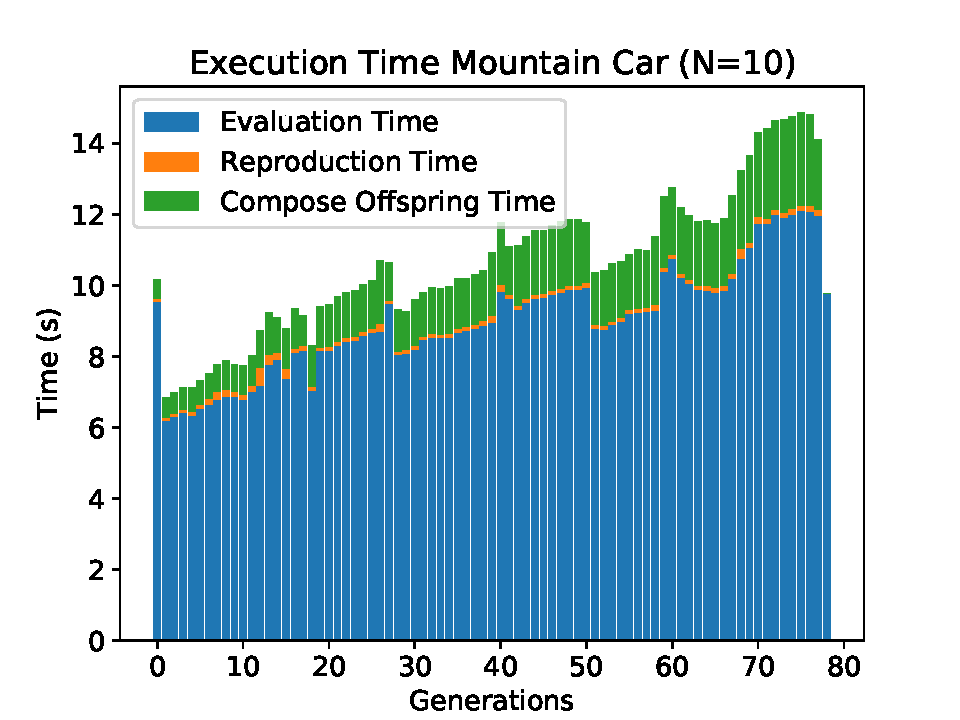
\includegraphics[width=0.9\textwidth]{./img/mountain_car_analysis/1413_time_10cores_10pis.pdf} 
	\caption{Ausführungszeit des \emph{MountainCar} Problems auf 10 Raspberry Pis mit 10 Prozessen}
	\label{fig:mountain_car_time_10cores_10pi}
\end{figure}
\\ \noindent
Im ersten Durchlauf wird der parallelisierte Algorithmus mit zehn Prozessen auf zehn Raspberry Pis ausgeführt. Das Verfahren ist so konfiguriert, dass auf jedem Raspberry Pi ein Prozess gestartet wird. Abbildung \ref{fig:mountain_car_10core_neural_network_and_fitness} zeigt das hierbei entstandene \ac{KNN} und den maximal erreichten Fitnesswert. Beide Darstellungen sind identisch mit denen des sequenziellen Verfahrens. Da auch die restlichen Zwischenergebnisse übereinstimmen, wie beispielsweise die Anzahl an verschiedenen Spezies pro Generation, ist die Anforderung bezüglich des \emph{Seeds} erfüllt. Sowohl die parallelisierte als auch die sequenzielle Implementierung führen dieselben Rechenschritte aus, wodurch ein direkter Vergleich der Laufzeiten möglich ist. Die Ausführungszeit für die vorgestellte Konfiguration ist in Abbildung  \ref{fig:mountain_car_time_10cores_10pi} dargestellt. Wie beim sequenziellen Verfahren wird diese in die Phasen \emph{Evaluation Time}, \emph{Reproduction Time} und \emph{Compose Offspring Time} unterteilt. Grundsätzlich ist festzustellen, dass die insgesamt benötigte Laufzeit stark verringert ist. Mit zehn Prozessen in der vorgestellten Konfiguration sinkt die durchschnittliche Rechenzeit auf ungefähr $10.5$ Sekunden pro Generation. Die sequenzielle Implementierung hat im Vergleich dazu etwa $80$ Sekunden pro Generation benötigt. Für die gesamte Ausführungszeit des Verfahrens bedeutet dies, dass das parallelisierte Verfahren bereits nach $14$ Minuten beendet ist. Im Vergleich zur Laufzeit der sequenziellen Implementierung mit $105$ Minuten ist das parallelisierte Verfahren $91$ Minuten schneller. Eine Besonderheit des Graphen zeigt sich in der ersten Generation. In dieser ist die Ausführungszeit der \emph{Evaluation Time} vergleichsweise hoch. Der Grund hierfür ist, dass das Starten und Initialisieren der beteiligten Prozesse Zeit benötigt, welche die Evaluation der Agenten verzögert. Da dies im Rahmen der \emph{Evaluation Time} erfasst wird, erhöht sich die gemessene Ausführungszeit in der ersten Generation. Für die nachfolgenden Generationen trifft dies nicht mehr zu, da die Initialisierung nur einmalig zu Beginn erfolgt. Eine weitere Besonderheit betrifft die Form des Graphen. Wie bei der sequenziellen Implementierung gibt es auch in der parallelisierten Implementierung Generationen, in denen die Ausführungszeit stark sinkt oder ansteigt. Mögliche Gründe hierfür sind in Kapitel \ref{subsec:analysis_mountain_car} erörtert. Bei einem direkten Vergleich der Ausführungszeiten ist festzustellen, dass diese Änderungen meistens in denselben Generationen auftreten. Diese Eigenschaft ist wichtig, da ein Vergleich der Laufzeiten nur möglich ist, wenn die Messergebnisse, von kleinen Abweichungen abgesehen, konsistent sind. Diese Eigenschaft kann zusätzlich mit der \emph{Reproduction Time} und \emph{Compose Offspring Time} verifiziert werden. Diese Phasen sind nicht parallelisiert und daher sollte die Ausführungszeit identisch sein. Insgesamt sind die gemessenen Laufzeiten in diesen Phasen etwas höher als bei der sequenziellen Implementierung. Über alle $78$ Generationen entsteht eine Differenz von ungefähr $5$ Sekunden beziehungsweise $4\%$. Diese Unterschiede können beispielsweise durch Hintergrundprozesse im Betriebssystem entstehen, auf welche kein Einfluss genommen werden kann. Da die Abweichungen insgesamt gering sind, kann dennoch ein Vergleich der Laufzeiten vorgenommen werden. Die letzte zu nennende Eigenschaft bezüglich der Abbildung \ref{fig:mountain_car_time_10cores_10pi} ist der prozentuale Anteil der \emph{Reproduction Time} und \emph{Compose Offspring Time}. Bei der sequenziellen Implementierung haben diese beiden Phasen nur etwa $2\%$ der Ausführungszeit in Anspruch genommen. Im aktuellen Testdurchlauf sind dies $15\%$, da durch die Parallelisierung der Anteil der \emph{Evaluation Time} sinkt. Aufgrund \emph{Amdahl's Law} ist anzunehmen, dass durch das Hinzufügen von weiteren Prozessen der prozentuale Anteil der \emph{Reproduction Time} und \emph{Compose Offspring Time} weiter ansteigt.
\begin{figure}[!h]
	\centering
	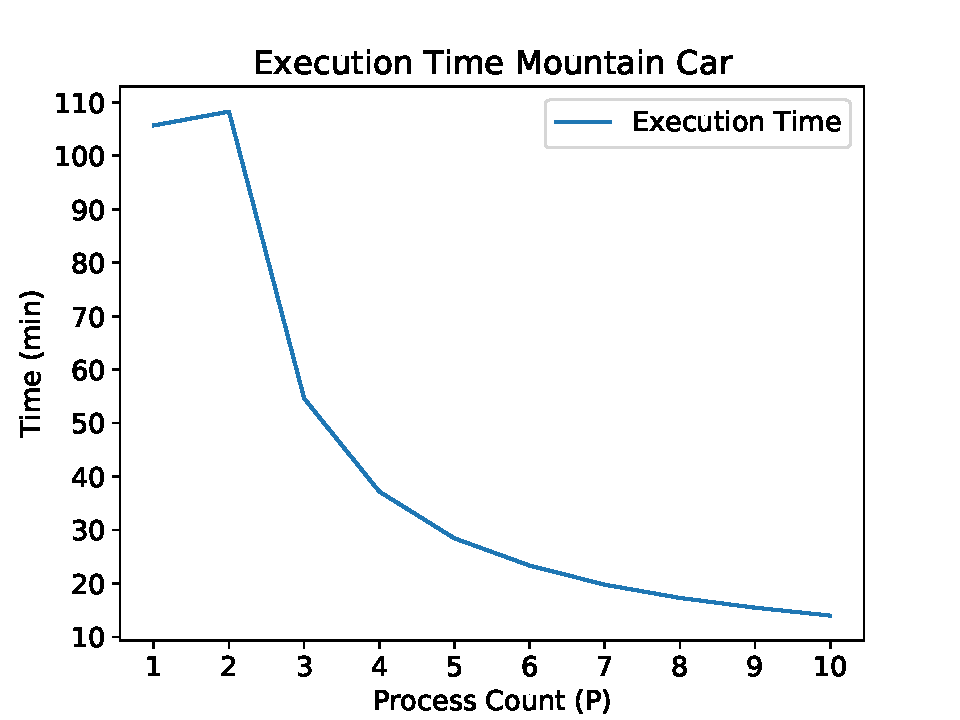
\includegraphics[width=0.7\textwidth]{./img/mountain_car_analysis/time_mountain_car_1_10.pdf} 
	\caption{Ausführungszeit des parallelisierten Verfahrens in der \emph{MountainCar} Umgebung in Abhängigkeit zur Prozessanzahl}
	\label{fig:execution_time_mountain_car_1_10}
\end{figure}
\\ \noindent
Für eine vollständige Bewertung des parallelisierten Verfahrens werden die in Kapitel \ref{subsec:basics_performance} vorgestellten Metriken \emph{SpeedUp} und Effizienz benötigt. Für eine bessere Einordnung der Ergebnisse werden diese nicht nur für die oben vorgestellte Konfiguration mit zehn Prozessen, sondern auch für Testdurchläufe mit zwei bis neun Prozessen berechnet. Diese werden im Folgenden mit derselben Konfiguration durchgeführt. Die hierbei entstehenden \ac{KNN} und Fitnesswerte sind identisch mit den vorherigen und sind daher nicht abgebildet. Die benötigte Ausführungszeit für das gesamte Verfahren in Abhängigkeit zur Anzahl an Prozessen ist in Abbildung \ref{fig:execution_time_mountain_car_1_10} dargestellt. Eine Besonderheit hierbei ist, dass die benötigte Ausführungszeit mit zwei Prozessen länger ist als die mit einem Prozess. Der Grund hierfür liegt in der gewählten \emph{Master-Slave} Architektur des parallelisierten Verfahrens. Mit einem Prozess wird das sequenzielle und andernfalls das parallelisierte Verfahren ausgeführt. Werden genau zwei Prozesse verwendet, gibt es einen \emph{Master} und einen \emph{Slave}. In diesem Fall ist die Ausführung langsamer als beim sequenziellen Verfahren, da der \emph{Master} im Rahmen der Parallelisierung nur die Kommunikation koordiniert, selbst aber keine Aufgabenpakete abarbeitet. Der \emph{Slave} führt alleine die Evaluation der Agenten durch. Dafür benötigt er dieselbe Zeit wie das sequenzielle Verfahren. Hinzu kommt der benötigte Kommunikationsaufwand für das Verteilen der Agenten und Sammeln von Fitnesswerten. Aufgrund der hierfür aufgewendeten Zeit ist das parallelisierte Verfahren mit zwei Prozessen langsamer als das sequenzielle Verfahren. Mit drei oder mehr beteiligten Prozessen sinkt die Ausführungszeit kontinuierlich. 
\begin{figure}[!h]
	\centering
	\begin{minipage}[]{0.49\textwidth}
		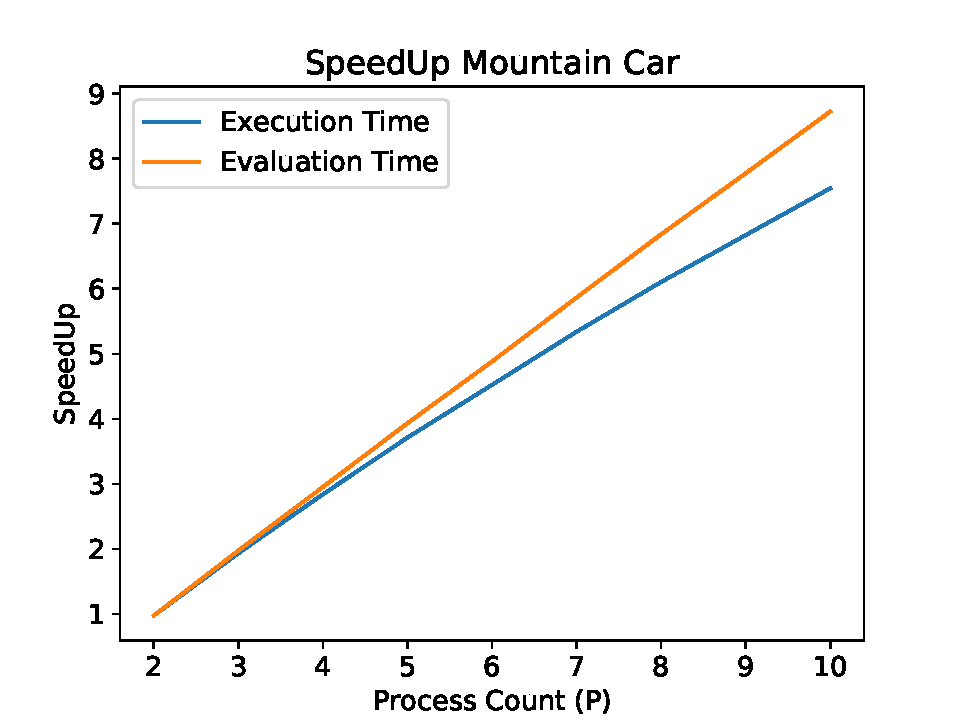
\includegraphics[width=1.0\textwidth]{./img/mountain_car_analysis/mountain_car_speedup_2_10.pdf} 
	\end{minipage}
	\hfill
	\begin{minipage}[]{0.49\textwidth}
		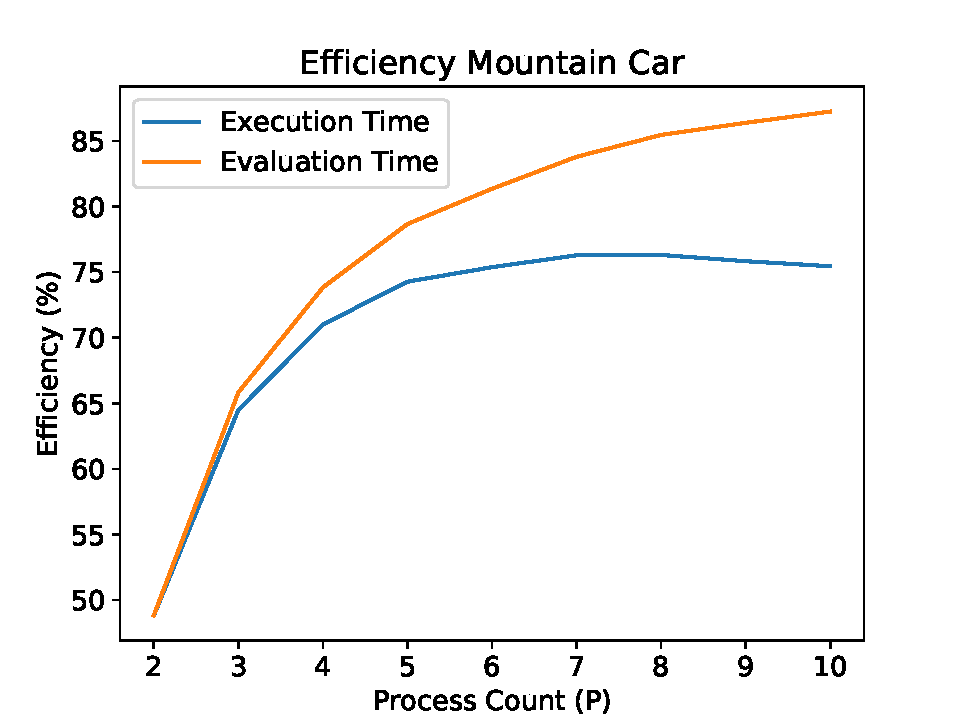
\includegraphics[width=1.0\textwidth]{./img/mountain_car_analysis/efficecny mountain_car_2_10.pdf} 
	\end{minipage}
	\caption{Links der \emph{SpeedUp}, rechts die dazugehörigen Effizienzwerte für die \emph{MountainCar} Umgebung in Abhängigkeit zur Prozessanzahl}
	\label{fig:mountain_car_2_10_efficiency_speedup}
\end{figure}
\\\\
Anhand der Ausführungszeiten wird der \emph{SpeedUp} und die Effizienz des parallelisierten Verfahrens gemessen, welche eine Bewertung der Implementierung ermöglichen. Abbildung \ref{fig:mountain_car_2_10_efficiency_speedup} zeigt links die erreichten \emph{SpeedUps} und rechts die dazugehörigen Effizienzwerte in Abhängigkeit zur Anzahl an verwendeten Prozessen. In beiden Graphen sind jeweils die Metriken für die Evaluationsphase und das gesamte Verfahren dargestellt. Beim Testdurchlauf mit zehn Prozessen ist das parallelisierte Verfahren ungefähr um den Faktor $7.6$ schneller als das sequenzielle Verfahren. Dieses Ergebnis ist grundsätzlich höher als bei den vorherigen Testdurchläufen mit weniger Prozessen, entspricht aber nicht der Vorhersage von \emph{Amdahl's Law}. Laut diesem liegt der maximal erreichbare \emph{SpeedUp} mit zehn Prozessen in einem zu $98\%$ parallelisierbaren Programm bei ungefähr $8.5$. Durch die gewählte \emph{Master-Slave} Kommunikationsarchitektur ist zwischen dem erwarteten und tatsächlich erhaltenen Wert eine Differenz von $0.9$. Wie bereits beschrieben, unterstützt der \emph{Master} die \emph{Slaves} nicht bei der Evaluation, wird aber dennoch bei den Berechnungen berücksichtigt. Wird nur die Anzahl der \emph{Slave} Prozesse bei der Berechnung von \emph{Amdahl's Law} verwendet, ergibt sich ein maximaler \emph{SpeedUp} von $7.8$. Die restliche Differenz von $0.2$ entsteht durch den Kommunikationsaufwand. 
\begin{figure}[!h]
	\centering
	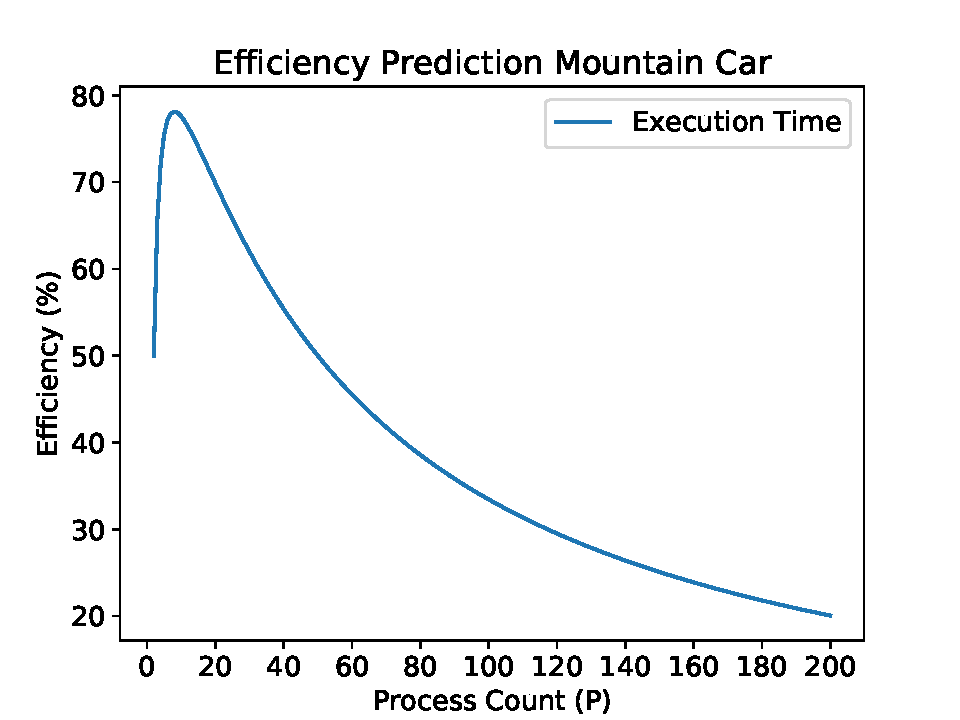
\includegraphics[width=0.7\textwidth]{./img/mountain_car_analysis/mountain_car_efficiency_prediction.pdf} 
	\caption{Erwartete Effizienz in der \emph{MountainCar} Umgebung in Abhängigkeit zur Anzahl an Prozessen}
	\label{fig:mountain_car_efficiency_predidction}
\end{figure}
\\ \noindent
Die in Abbildung \ref{fig:mountain_car_2_10_efficiency_speedup} rechts dargestellten Effizienzwerte beurteilen den \emph{SpeedUp} anhand der Prozessanzahl. Initial erzielt das parallelisierte Verfahren mit zwei Prozessen aufgrund der \emph{Master-Slave} Architektur eine geringe Effizienz. Mit je einem \emph{Master} und \emph{Slave} wird entsprechend der Abbildung \ref{fig:execution_time_mountain_car_1_10} eine etwas höhere Ausführungszeit im Vergleich zur sequenziellen Implementierung benötigt. Daher liegt der \emph{SpeedUp} bei ungefähr $0.98$. Entsprechend der Formel aus Kapitel \ref{subsec:basics_performance} ergibt die Berechnung der Effizienz einen Wert von $49\%$. Beim Hinzufügen weiterer Prozesse sinkt der Einfluss des \emph{Masters} auf das Ergebnis und die Effizienz steigt. Mit sechs bis zehn Prozessen wird ein Wert von über $75\%$ erreicht. Aufgrund des Graphen und \emph{Amdahl's Law} ist davon auszugehen, dass der Wert nicht weiter steigen, sondern durch Hinzufügen weiterer Prozesse letztendlich sinken wird. Abbildung \ref{fig:mountain_car_efficiency_predidction} zeigt die erwarteten Effizienzwerte für die \emph{MountainCar} Umgebung mit einer \emph{Master-Slave} Architektur, wobei die Werte mit \emph{Amdahl's Law} berechnet worden sind. Auch in diesem Fall steigt die Effizienz anfangs stark an. Der höchste Wert von ungefähr $78\%$ wird mit acht Prozessen erreicht. Dies entspricht etwa dem tatsächlich erhaltenen Ergebnis. Hierbei wird die höchste Effizienz von $76\%$ ebenfalls mit acht Prozessen erreicht. Der Grund für das starke Absinken der Effizienz im weiteren Verlauf ist darin begründet, dass der \emph{SpeedUp} durch den sequenziellen Anteil von \emph{Amdahl's Law} immer gegen einen bestimmten Wert konvergiert. Die niedrigen Effizienzwerte entstehen, da der \emph{SpeedUp} nicht proportional zur Anzahl der Prozesse ansteigt.
\\\\
Es ist möglich, den \emph{SpeedUp} und die Effizienz nur für die parallelisierte \emph{Evaluation Time} zu berechnen, sodass der sequenzielle Teil des Verfahrens keinen Einfluss auf das Ergebnis hat. Die Ergebnisse hiervon sowie die des gesamten Verfahrens sind in Abbildung \ref{fig:mountain_car_2_10_efficiency_speedup} dargestellt. Der \emph{SpeedUp} der \emph{Evaluation Time} ist nahezu linear. Mit neun \emph{Slaves} bzw. zehn Prozessen wird ein \emph{SpeedUp} von $8.7$ erreicht. Diese guten Ergebnisse spiegeln sich in der Effizienz wieder. Diese ist anfänglich durch die \emph{Master-Slave} Architektur bei $49\%$, steigt aber stetig an. Mit zehn Prozessen liegt sie bei $87\%$. Prinzipiell kann der Wert weiter ansteigen, da der Einfluss des \emph{Masters} auf das Ergebnis mit zunehmender Prozessanzahl sinkt. Dennoch ist aufgrund der entstehenden Kommunikationszeit keine Effizienz von $100\%$ möglich. Bleibt bei der Effizienzberechnung der \emph{Master} Prozess unberücksichtigt, werden Ergebnisse zwischen $97\%$ und fast $99\%$ erreicht. Dies entspricht nahezu dem idealen Wert.

\subsection{Pendulum}
In diesem Kapitel wird die \emph{Pendulum} Umgebung mit dem parallelisierten Verfahren evaluiert und bewertet. Zusätzlich erfolgt ein Vergleich mit den Ergebnissen des vorherigen Kapitels. Hierzu wird das Optimierungsproblem zunächst in verschiedenen Testdurchläufen mit zwei bis zehn Prozessen optimiert und jeweils die \emph{Evaluation Time}, \emph{Reproduction Time} und \emph{Compose Offspring Time} erfasst. Die Konfiguration und der \emph{Seed} werden vom sequenziellen Verfahren übernommen, sodass alle Testdurchläufe dieselben Lösungen produzieren und ein Vergleich der Implementierungen möglich ist. Wie bei der \emph{MountainCar} Umgebung wird von jedem Raspberry Pi maximal ein Prozess ausgeführt. 
\begin{figure}[!htb]
	\centering
	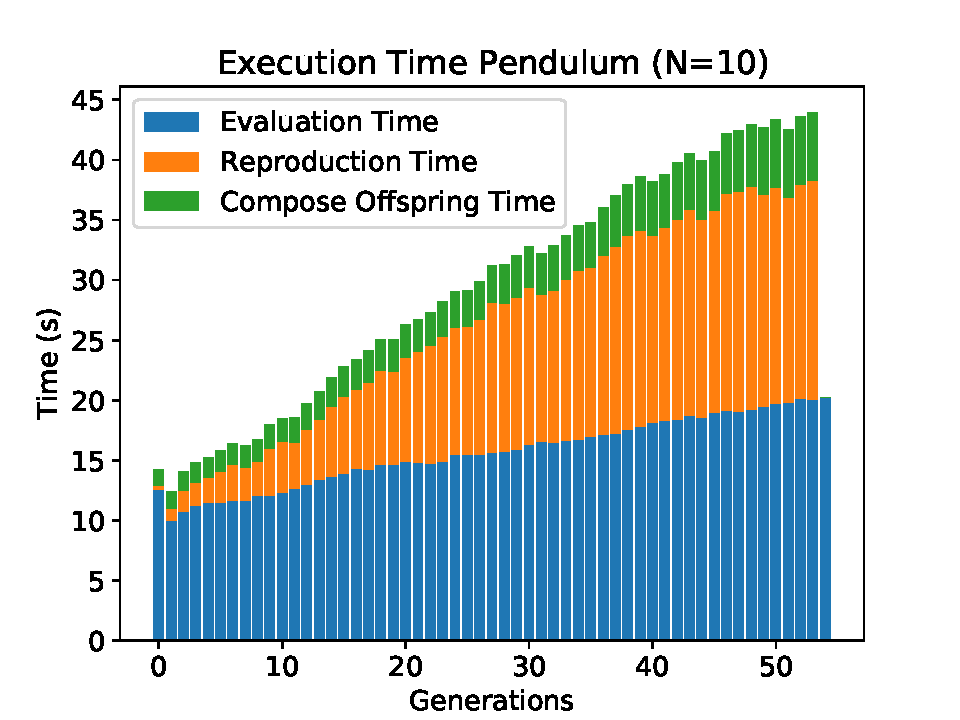
\includegraphics[width=0.9\textwidth]{./img/pendulum_analysis/pendulum_time_1_10core_10pi.pdf} 
	\caption{Ausführungszeit des \emph{Pendulum} Problems auf 10 Raspberry Pis mit 10 Prozessen}
	\label{fig:pendulum_time_10cores_10pi}
\end{figure}
\\\\
Die Ergebnisse zeigen, dass die Fitnesswerte und die finalen \ac{KNN} identisch mit denen des sequenziellen Verfahrens sind, daher wird auf eine Abbildung verzichtet. Der Schwerpunkt der Analyse liegt auf den Ausführungszeiten. Diese sind von dem zuletzt durchgeführten Test mit zehn Prozessen in Abbildung \ref{fig:pendulum_execution_time_1_10} dargestellt. Wie bei der \emph{MountainCar} Umgebung ist die \emph{Evaluation Time} der ersten Generation höher als die der zweiten. Der Grund hierfür liegt in der Initialisierung der einzelnen Prozesse. Die gesamte Ausführungszeit in diesem Test beträgt $27$ Minuten. Verglichen mit der Ausführungszeit der sequenziellen Implementierung von 138 Minuten ist dies eine Zeitersparnis von $111$ Minuten. Zuletzt ist bezüglich dieses Graphen hervorzuheben, dass die \emph{Evaluation Time} im Verlauf der Generationen nur leicht ansteigt und insgesamt $53\%$ der Ausführungszeit ausmacht. Der Anteil der beiden anderen Phasen ist anfänglich gering, steigt aber stark an und benötigt zusammen in den letzten Generationen mehr Zeit als die eigentliche Evaluation. Wie bereits beim sequenziellen Verfahren beschrieben, ist die hohe Anzahl an verschiedenen Spezies der Grund für die vergleichsweise hohe \emph{Reproduction Time}.
\begin{figure}[!htb]
	\centering
	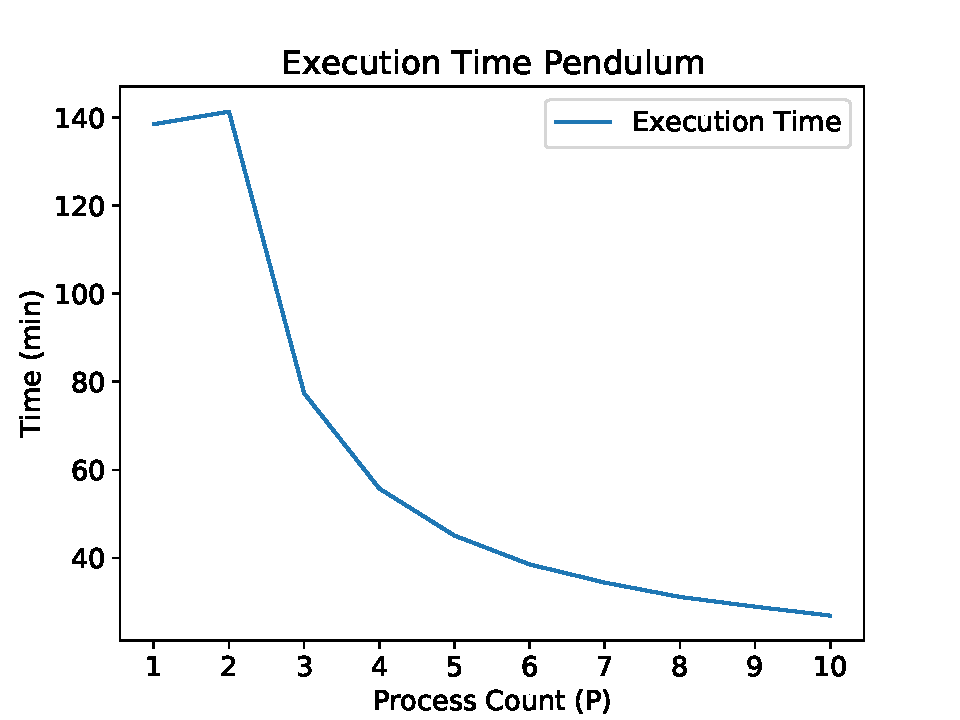
\includegraphics[width=0.7\textwidth]{./img/pendulum_analysis/pendulum_execution_1_1_10.pdf} 
	\caption{Ausführungszeit des parallelisierten Verfahrens in der \emph{Pendulum} Umgebung in Abhängigkeit zur Prozessanzahl}
	\label{fig:pendulum_execution_time_1_10}
\end{figure}
\\\\
Als nächstes wird der Verlauf der gesamten Ausführungszeit in Abhängigkeit zur Anzahl an Prozessen betrachtet. Diese sind in Abbildung \ref{fig:pendulum_execution_time_1_10} dargestellt. Prinzipiell ähnelt der Graph dem der \emph{MountainCar} Evaluation. Mit zwei Prozessen steigt die Ausführungszeit im Vergleich zum sequenziellen Verfahren an. Wie in Kapitel \ref{subsec:mountain_car_optimzation} beschrieben, ist der Grund hierfür die gewählte \emph{Master-Slave} Architektur. Mit steigender Anzahl an Prozessen nimmt die Ausführungszeit kontinuierlich ab. Gegen Ende wird die Zeitersparnis mit zunehmender Anzahl an Prozessen immer geringer. Grund hierfür sind die sequenziellen Phasen des Verfahrens. 
\begin{figure}[!htb]
	\centering
	\begin{minipage}[]{0.49\textwidth}
		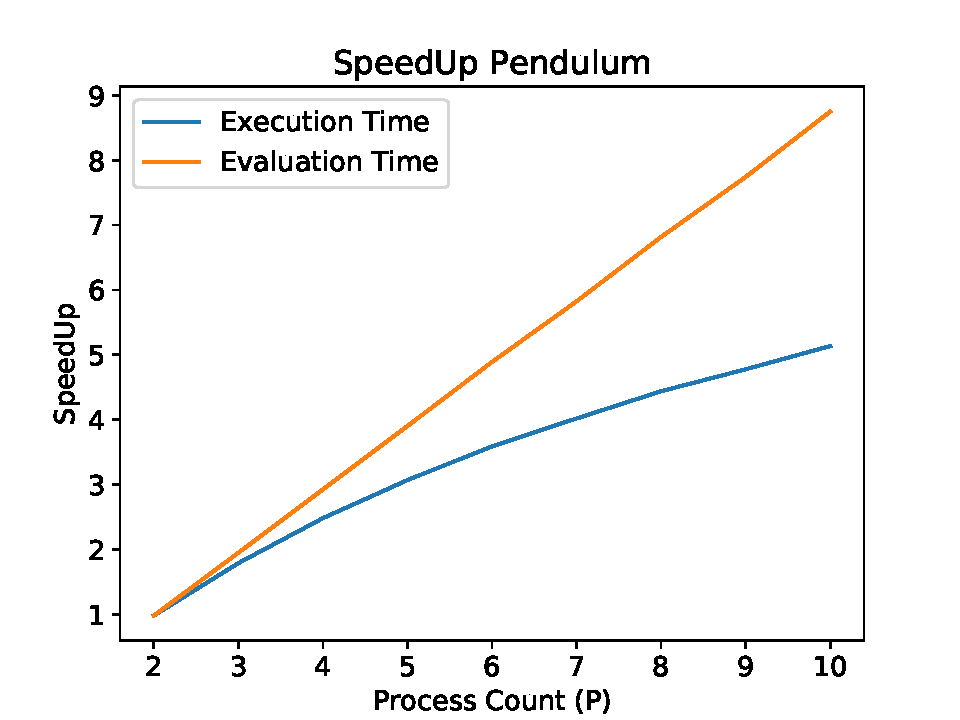
\includegraphics[width=1.0\textwidth]{./img/pendulum_analysis/pendulum_speedup1_2_10.pdf} 
	\end{minipage}
	\hfill
	\begin{minipage}[]{0.49\textwidth}
		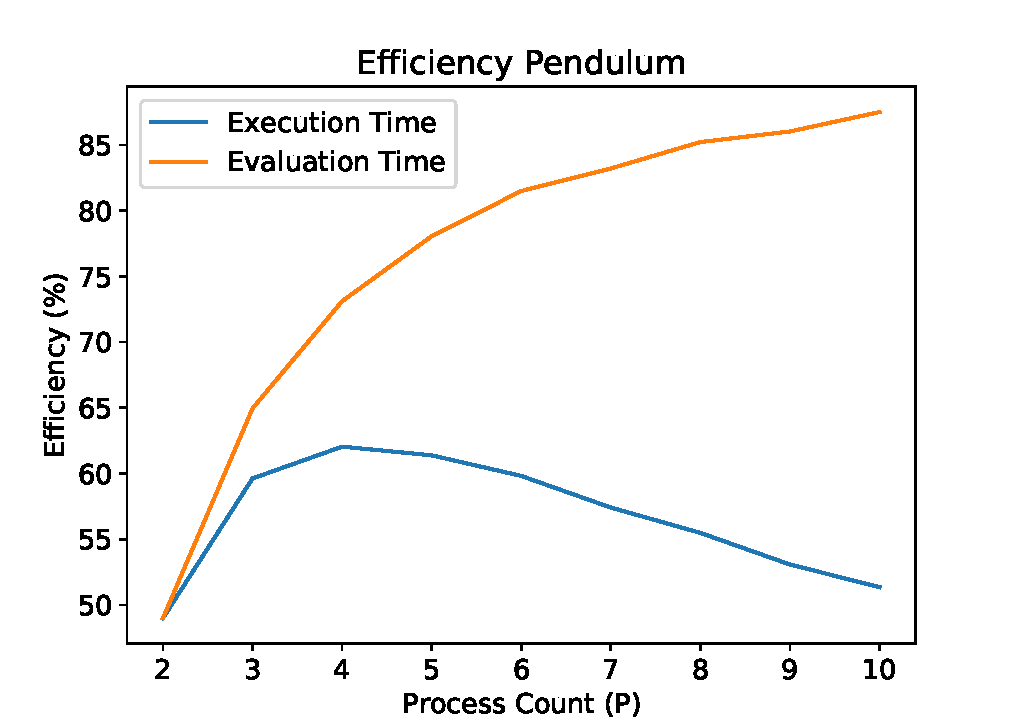
\includegraphics[width=1.0\textwidth]{./img/pendulum_analysis/efficiency_pendulum_2_10.pdf} 
	\end{minipage}
	\caption{Links der \emph{SpeedUp}, rechts die dazugehörigen Effizienzwerte für die \emph{Pendulum} Umgebung in Abhängigkeit zur Prozessanzahl}
	\label{fig:pendulum_2_10_efficiency_speedup}
\end{figure}
\\\\
Um die Ausführungszeiten und den Grad der Parallelisierung besser bewerten zu können, wird der \emph{SpeedUp} und die Effizienz für jeden Durchlauf berechnet. Die Ergebnisse sind in Abbildung \ref{fig:pendulum_2_10_efficiency_speedup} dargestellt, wobei jeweils die Werte für das gesamte Verfahren und die parallelisierte \emph{Evaluation Time} dargestellt sind. Auf Letzteres wird zuerst eingegangen. Der \emph{SpeedUp} für die Evaluationsphase ist nahezu konstant. Mit zehn Prozessen wird ein Faktor von $8.75$ erzielt. Dieses Ergebnis ähnelt dem der \emph{MountainCar} Umgebung, bei der in dieser Phase ein Faktor von $8.7$ erreicht wird. Das Ergebnis ist insgesamt als sehr gut zu bewerten, da in der \emph{Master-Slave} Architektur mit zehn Prozessen bzw. neun \emph{Slaves} der maximal erreichbare \emph{SpeedUp} $9$ beträgt. Dies spiegelt sich auch in der Effizienz wieder. Bei der \emph{Master-Slave} Architektur liegt diese initial bei $49\%$, steigt aber stetig an. Mit zehn Prozessen wird ein Wert von $87\%$ für die Parallelisierung der \emph{Evaluation Time} erzielt. Die vergleichsweise schlechten initialen Messwerte sind durch die Berücksichtigung des \emph{Masters} bei der Berechnung zu erklären, da er selbst keine Agenten evaluiert. Derselbe Umstand tritt in der \emph{MountainCar} Umgebung auf. Werden bei der Berechnung nur die zur Verfügung stehenden \emph{Slaves} betrachtet, liegt die Effizienz in allen Testdurchläufen bei ungefähr $97\%$, maximal bei $98\%$. Aufgrund der notwendigen Kommunikation wird keine Effizienz von $100\%$ erreicht. Zusammengefasst zeigen diese Ergebnisse, dass die Parallelisierung der \emph{Evaluation Time} in beiden Testdurchläufen sehr gute und konstante Ergebnisse liefert. Es ist davon auszugehen, dass trotz Hinzufügen von weiteren Prozessen die Effizienz bei einer entsprechenden Populationsgröße weiterhin hoch ist. Hierauf wird im Rahmen der Ergebnisse in Kapitel \ref{sec:results_optimziation} genauer eingegangen. In Abbildung \ref{fig:pendulum_2_10_efficiency_speedup} sind nicht nur der \emph{SpeedUp} und die Effizienz für die Evaluationsphase, sondern auch das gesamten Verfahrens dargestellt. Die hierbei erhaltenen Werte sind nicht so gut wie in der \emph{MountainCar} Umgebung. Mit zehn Prozessen wird ein \emph{SpeedUp} von $5.1$ erreicht. Die \emph{MountainCar} Umgebung erzielt im Vergleich hierzu noch einen Wert von $7.6$. Auch der Anstieg des \emph{SpeedUps} sinkt innerhalb der ersten zehn Generationen drastisch. Grund hierfür ist der Anteil der nicht parallelisierten \emph{Reproduction Time} und \emph{Compose Offspring Time}. Wie in Kapitel \ref{sec:parallel_strategies} veranschaulicht, ist in der \emph{Pendulum} Umgebung ein maximaler \emph{SpeedUp} von $11.\overline{1}$ möglich. Mit steigender Anzahl an Prozessen nähert sich das Ergebnis diesem Wert an.
\\\\
Entsprechend des \emph{SpeedUps} sind auch die Effizienzwerte weniger gut als in der \emph{MountainCar} Umgebung. Anfangs liegt diese bei $42\%$, steigt danach an, erreicht mit vier Prozessen das Maximum von $62\%$ und sinkt danach kontinuierlich. Hierfür sind dieselben Gründe maßgeblich wie in der \emph{MountainCar} Umgebung. Um die erhaltenen Ergebnisse besser einordnen zu können, werden mit \emph{Amdahl's Law} die zu erwartenden Effizienzwerte berechnet. Diese sind in Abbildung \ref{fig:pendulumr_efficiency_predidction} dargestellt. Aufgrund der unterschiedlichen Skalierung an den Achsen ist nicht offensichtlich, dass die gemessenen und idealen Ergebnisse sehr ähnlich sind. Die maximal erreichbare Effizienz von ungefähr $63.5\%$ tritt ebenfalls mit vier Prozessen auf. Die übrigen Effizienzwerte für zwei bis zehn Prozesse weichen weniger als zwei Prozentpunkte vom tatsächlich erhaltenen Ergebnis ab. 
\begin{figure}[!h]
	\centering
	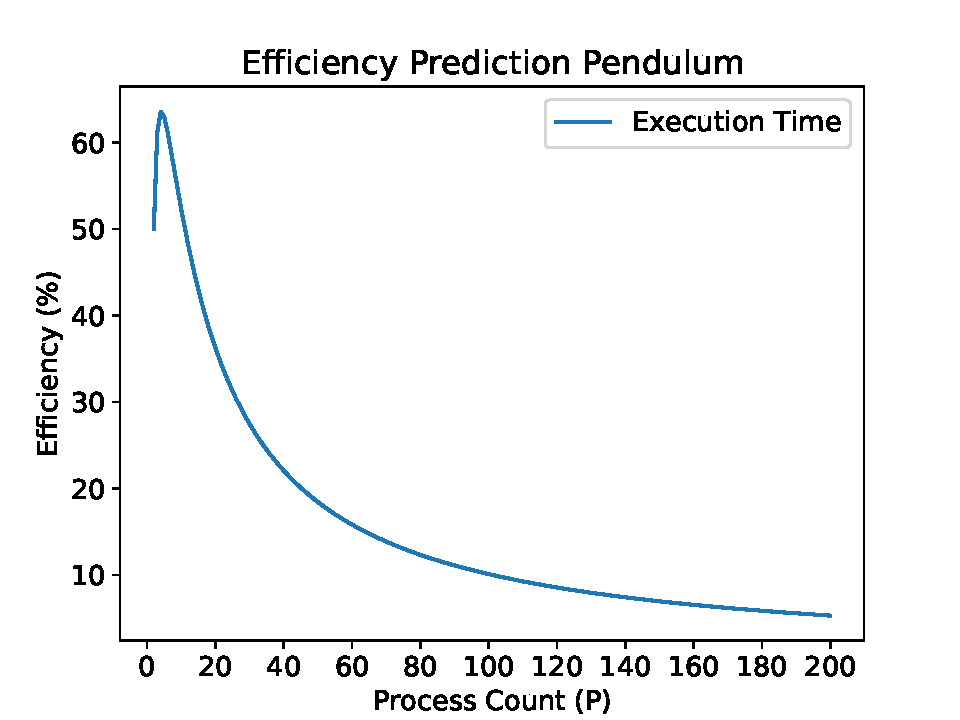
\includegraphics[width=0.7\textwidth]{./img/pendulum_analysis/pendulum_efficiency_prediction.pdf} 
	\caption{Erwartete Effizienz in der \emph{Pendulum} Umgebung in Abhängigkeit zur Anzahl an Prozessen}
	\label{fig:pendulumr_efficiency_predidction}
\end{figure}

\subsection{Multi-Core CPUs}
Die bisherigen Testdurchläufe nutzen maximal zehn Prozesse gleichzeitig, und zwar einen auf jedem Raspberry Pi. Mit dieser Konfiguration werden insgesamt sehr gute \emph{SpeedUp} Ergebnisse erzielt. Prinzipiell ist es mit der bereits vorhandenen Hardware möglich, die Ausführungszeit weiter zu reduzieren, da die \ac{CPU} der einzelnen Raspberry Pis nicht vollständig ausgelastet ist. Grund hierfür sind die Hardware und Funktionsweise der Programmiersprache Python. Wie in Kapitel \ref{sec:analysis_testsetup} beschrieben, verfügt der Raspberry Pi 4 über einen Quad-core ARM Prozessor. Das bedeutet, dass sich vier unabhängige Prozessoren auf derselben \ac{CPU} befinden, die parallel Instruktionen ausführen können. Allerdings kann der Standard Python Interpreter dies nicht nutzen, da ein \ac{GIL} verwendet wird, um die Sprache \emph{thread-safe} zu machen. Das bedeutet, dass nur ein \emph{Thread} gleichzeitig ausgeführt werden kann. Existieren mehrere \emph{Threads} wechselt der Python Interpreter in regelmäßigen Abständen zwischen diesen, sodass jedem eine gewisse Ausführungszeit zukommt. Die Folge ist, dass alle \emph{Threads}, eines Programms auf demselben Prozessor abgearbeitet werden und keine Reduzierung der Ausführungszeit möglich ist \cite{marowka2018python}. Für das Umgehen des \acp{GIL} gibt es verschiedene Ansätze, wobei eine Möglichkeit das Nutzen von \ac{MPI} ist. Die parallelisierte Implementierung kann in der vorgestellten Testumgebung auf zehn Raspberry Pis mit insgesamt $40$ Prozessen gestartet werden, sodass jeder Raspberry Pi vier Prozesse zugewiesen bekommt. Das Betriebssystem verteilt diese auf die vier verfügbaren Prozessoren und erzielt so eine parallele Ausführung. Bei dieser Umsetzung verfügen die einzelnen Prozesse jeweils über einen eigenen \ac{GIL}, der jedoch nicht mit denen von anderen Prozessen interferiert.
\begin{figure}[!h]
	\centering
	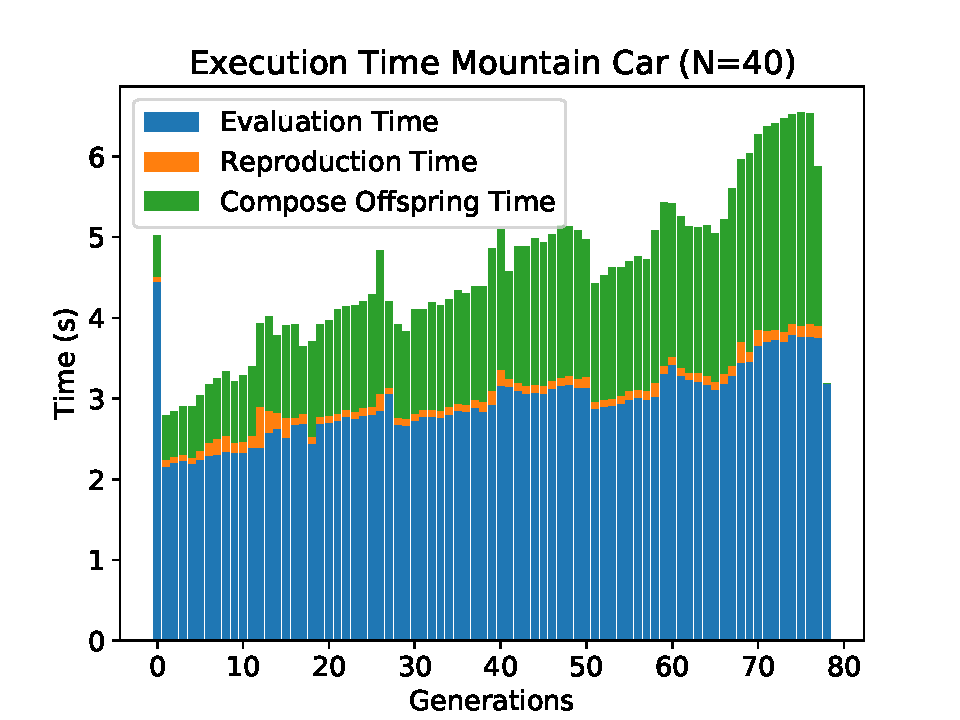
\includegraphics[width=0.9\textwidth]{./img/mountain_car_analysis/1413_time_40core_10pi.pdf} 
	\caption{Ausführungszeit des \emph{MountainCar} Problems auf 10 Raspberry Pis mit 40 Prozessen}
	\label{fig:mountain_car_time_40core_10pi}
\end{figure}
\\\\
Um die Performance von diesem Szenario zu testen, werden die \emph{MountainCar} und \emph{Pendulum} Umgebung erneut ausgeführt. Aufgrund der vorherigen Ergebnisse ist zu erwarten, dass die Ausführungszeit der \emph{Evaluation Time} ungefähr um den Faktor vier im Vergleich zu zehn Prozessen verringert wird. Abweichungen können durch andere Hintergrundprozesse oder das Betriebssystem entstehen, mit denen die verfügbaren Rechenkapazitäten geteilt werden müssen. Abbildung \ref{fig:mountain_car_time_40core_10pi} zeigt die gemessenen Ausführungszeiten für die \emph{MountainCar} Umgebung mit $40$ Prozessen. Diese ist grundsätzlich im Vergleich zu den vorherigen Testdurchläufen gesunken. Insgesamt werden etwa sechs Minuten für die gesamte Ausführung benötigt, dies entspricht einer Zeitersparnis von $99$ Minuten gegenüber dem sequenziellen Verfahren. Im Vergleich zu dem Testdurchlauf mit zehn Prozessen ist die Ausführungszeit um 8 Minuten gesunken. Um eine Bewertung der Parallelisierung zu ermöglichen, wird der \emph{SpeedUp} und die Effizienz für das gesamte Verfahren sowie die \emph{Evaluation Time} berechnet.  Der \emph{SpeedUp} für das gesamte Verfahren beträgt im Vergleich zur sequenziellen Implementierung ungefähr $17.6$, die Effizienz liegt bei $44\%$. Diese Ergebnisse entsprechen nicht den Erwartungen. Nach \emph{Amdahl's Law} soll ein \emph{SpeedUp} von ungefähr $22.5$ erzielt werden, beziehungsweise von $22.1$, wenn der \emph{Master} Prozess bei der Berechnung nicht berücksichtigt wird. Bei Betrachtung der \emph{Evaluation Time} sind die erhaltenen  Ergebnisse ebenfalls geringer als erwartet. Für diese Phase wird ein \emph{SpeedUp} von $26.7$ erzielt, was einer Effizienz von ungefähr $67\%$ entspricht. Selbst wenn der \emph{Master} Prozess keine Berücksichtigung findet und ausschließlich die \emph{Slaves} betrachtet werden, liegt die Effizienz nur bei $68.4\%$. Dieses Ergebnis ist bedeutend geringer als die mit zwei bis zehn Prozessen erreichte Effizienz $97\%$ bis $99\%$. Auch wenn bei der \emph{Pendulum} Umgebung etwas bessere Ergebnisse erzielt werden, skaliert die Leistung nicht wie erwartet. Der \emph{SpeedUp} für die \emph{Evaluation Time} beträgt ungefähr $29.6$ und ergibt eine Effizienz von $74\%$, beziehungsweise $76\%$, wenn der \emph{Master} nicht in die Berechnung miteinbezogen wird. Auch dies liegt über $20$ Prozentpunkte unter den vorherigen Ergebnissen. 
\\\\
Für den Leistungseinbruch können verschiedene Faktoren ursächlich sein. Offensichtlich ist, dass an einer Stelle des Systems ein Ressourcenengpass entsteht. Um den Grund hierfür zu lokalisieren, werden verschiedene Tests durchgeführt, auf deren Ergebnisse im Folgenden eingegangen wird. Zuerst wird der \emph{Master} Prozess untersucht. Dieser muss die Arbeitspakete mit einer geringen Latenz verteilen, sodass die \emph{Slaves} geringe Wartezeiten haben. Aufgrund der hohen Anzahl an Prozessen ist dies unter Umständen nicht gewährleistet. Um diese These zu prüfen, wird das Optimierungsproblem angepasst. Jeder Agent muss bei der Evaluierung dieselbe Umgebung zehnmal absolvieren. Dies ändert nicht das Ergebnis, erhöht aber die Ausführungszeit stark. Zwar ist die hierbei entstehende Last auf den \emph{Master} unverändert, sie wird jedoch über eine größere Zeitspanne verteilt. Falls beim \emph{Master} Prozess der Ressourcenengpass auftritt, müsste durch diese Maßnahme eine Steigerung der Effizienz erkennbar sein. Dies ist jedoch nicht der Fall. Die Ergebnisse zeigen nur eine geringfügige Steigerung. Daher kann der \emph{Master} Prozess als Engpass der Implementierung ausgeschlossen werden. 
\\\\
Als nächstes wird die Hard- bzw. Software des Beowulf-Clusters überprüft, wobei der nächste Test verifiziert, ob der Ressourcenengpass bei den einzelnen \emph{Nodes} entsteht. Hierzu werden neun Prozesse auf drei Raspberry Pis ausgeführt, wobei auf einem Gerät der \emph{Master} Prozess und auf den anderen jeweils vier \emph{Slave} Prozesse gestartet werden. Mit dieser Konfiguration beträgt die Ausführungszeit des Verfahrens fast $20$ Minuten und ein \emph{SpeedUp} von $5.3$ wird erzielt. Der Anteil der \emph{Evaluation Time} beträgt hierbei $17.7$ Minuten. Diese Werte sind im Vergleich zum Durchlauf auf neun Raspberry Pis substanziell schlechter. Trotz derselben Anzahl an Prozessen ist die benötigte Ausführungszeit für das gesamte Verfahren um $28\%$ höher und somit um $4.4$ Minuten langsamer. Bei der Pendulum Umgebung treten ähnliche Ergebnisse auf. Daraus lässt sich folgern, dass mehrere Prozesse auf demselben Raspberry Pi sich teilweise gegenseitig blockieren und dadurch eine längere Ausführungszeit entsteht. 
\\\\
Zuletzt ist festzustellen, durch welche Komponenten des Algorithmus die Verzögerung entsteht. In einem ersten Schritt wird eine Umgebung des\emph{OpenAI Gyms} untersucht. Abbildung \ref{fig:test_bottleneck} zeigt den erstellten Test. Es wird zuerst die \emph{Pendulum} Umgebung initialisiert und danach $160.000$ Zufallsaktionen ausgeführt. Die hierfür benötigte Zeit wird gemessen und am Ende dargestellt. Der Test wird zunächst mit einem Prozess ausgeführt, dabei wird eine Laufzeit von $75.6$ Sekunden gemessen. Danach wird der Test mit vier Prozessen auf einem Raspberry Pi wiederholt. Der zu leistende Rechenaufwand wird in diesem Fall nicht geteilt. Daher sollte jeder Prozess $160.000$ Zufallsaktionen in einer lokalen Umgebung ausführen und dafür dieselbe Zeit benötigten. Allerdings zeigen die Messergebnisse einen Anstieg von $27\%$ auf $95.5$ Sekunden. Ein vergleichbarer Test wird mit einem \ac{KNN} durchgeführt. Mit einem Prozess werden hierfür $73$ Sekunden benötigt. Beim der Ausführung mit vier Prozessen steigt die Laufzeit um ungefähr $9.5\%$ auf 80 Sekunden an. Da in den letzten beiden Tests keine Nachrichten ausgetauscht werden, ist zu schlussfolgern, dass die zuvor festgestellten Leistungseinbrüche mit $40$ Prozessen nicht durch einen zu großen Kommunikationsaufwand, sondern vor allem durch die verwendeten Optimierungsprobleme entstehen. 
\begin{figure}
	\begin{python}
		import gym
		import time
		
		env = gym.make("Pendulum-v0")
		env.reset()
		
		start_time = time.time()
		for _ in range(160000):
			env.step(env.action_space.sample())
		
		time_required = time.time() - start_time
		print(time_required)
	\end{python}
	\label{fig:test_bottleneck}
	\caption{Python Programmcode zum Überprüfen der Parallelisierung des \emph{OpenAI Gyms}}
\end{figure} 


% Prozentsatz an Abweidung nicht parllelisierter Verfahren, 
% Zuerst Ergebnisse 10 Pis, mit Verifizierung Funktionalität und allgemeines Ergebnis
% Eingehen dass Master Pi keine Abarbeitugn übernimmt sondern nur Koordination
% Zeiten von anderen Phasen weichen ab, daher kann es zu varianzen kommen
% Allgemeine Laufzeit des Verfahrens und Laufzeit des evaluierten Verfahren anzeigen
% Vergleich mit Amdahls Law? +++++ 
